\documentclass[10pt]{beamer}

\usetheme[progressbar=frametitle, numbering=fraction,]{metropolis}

\usepackage{booktabs}
\usepackage{pgfplots}
\usepgfplotslibrary{dateplot}
\usepackage{texshade}      
\usepackage{amsmath}
\usepackage{amssymb}
\usepackage{xspace}
\usepackage{xcolor}
\usepackage{tikz}
\usepackage{forest}
\usepackage{verbatim}
\usepackage{appendixnumberbeamer}

\usetikzlibrary{arrows.meta}

\newcommand{\highlight}[1]{%
  \colorbox{yellow!50}{$\displaystyle#1$}}
  
\newcommand{\themename}{\textbf{\textsc{metropolis}}\xspace}
\newcommand{\red}[1]{\textcolor{red}{#1}}
\newcommand{\blue}[1]{\textcolor{blue}{#1}}
\newcommand{\green}[1]{\textcolor{green}{#1}}
\newcommand{\yellow}[1]{\textcolor{yellow}{#1}}

\setbeamercovered{invisible}
\setbeamertemplate{caption}{\raggedright\insertcaption\par}

\title{Modeling evolution of transcription factor binding sites}
%: \textit{Evolutionary} Ideas}
\subtitle{}
\date{\today}
\author{Saket Choudhary}
%\institute{Center for modern beamer themes}
%\titlegraphic{\hfill
\includegraphics[height=1.5cm]{logo}}

\begin{document}

\maketitle

\begin{frame}{Table of contents}
  \setbeamertemplate{section in toc}[sections numbered]
  \tableofcontents[hideallsubsections]
\end{frame}

\section{Introduction}
{
\setbeamertemplate{frame footer}{Wasserman, W. W., \& Sandelin, A. (2004)}
\begin{frame}[fragile]{TFs bind to specific sets of short sequences}
  \begin{figure}
	  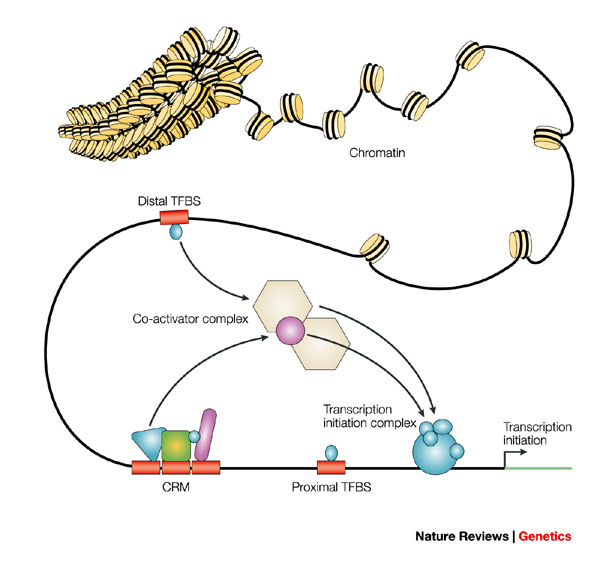
\includegraphics[width=0.8\linewidth]{images/crm.jpg}
  \end{figure}
\end{frame}
}

\begin{frame}[fragile]{TFBS: Properties}
  \begin{columns}[T,onlytextwidth]
    \column{0.5\textwidth}
    \begin{itemize}[<+- | alert@+>]
    	\item Short sequences (5-25bp)
  	  	\item Proximity to TSS (~100-1000bp)
   		\item Degeneracy
        %\item Under selection
    \end{itemize}
	\column{0.5\textwidth}
	\begin{texshade}{images/aln-msf.txt}
      \setends{1}{1..5}
      \hidenumbering
      \showsequencelogo{top}
      \showconsensus[ColdHot]{bottom}
      \defconsensus{.}{lower}{upper}
	\end{texshade}
  \end{columns}
\end{frame}


\section{Separation of mutability and selection}

{
\setbeamertemplate{frame footer}{Tagle et al. (1988)}

\begin{frame}[fragile]{Phylogenetic footprinting for identifying regulatory elements}
      \begin{figure}
      	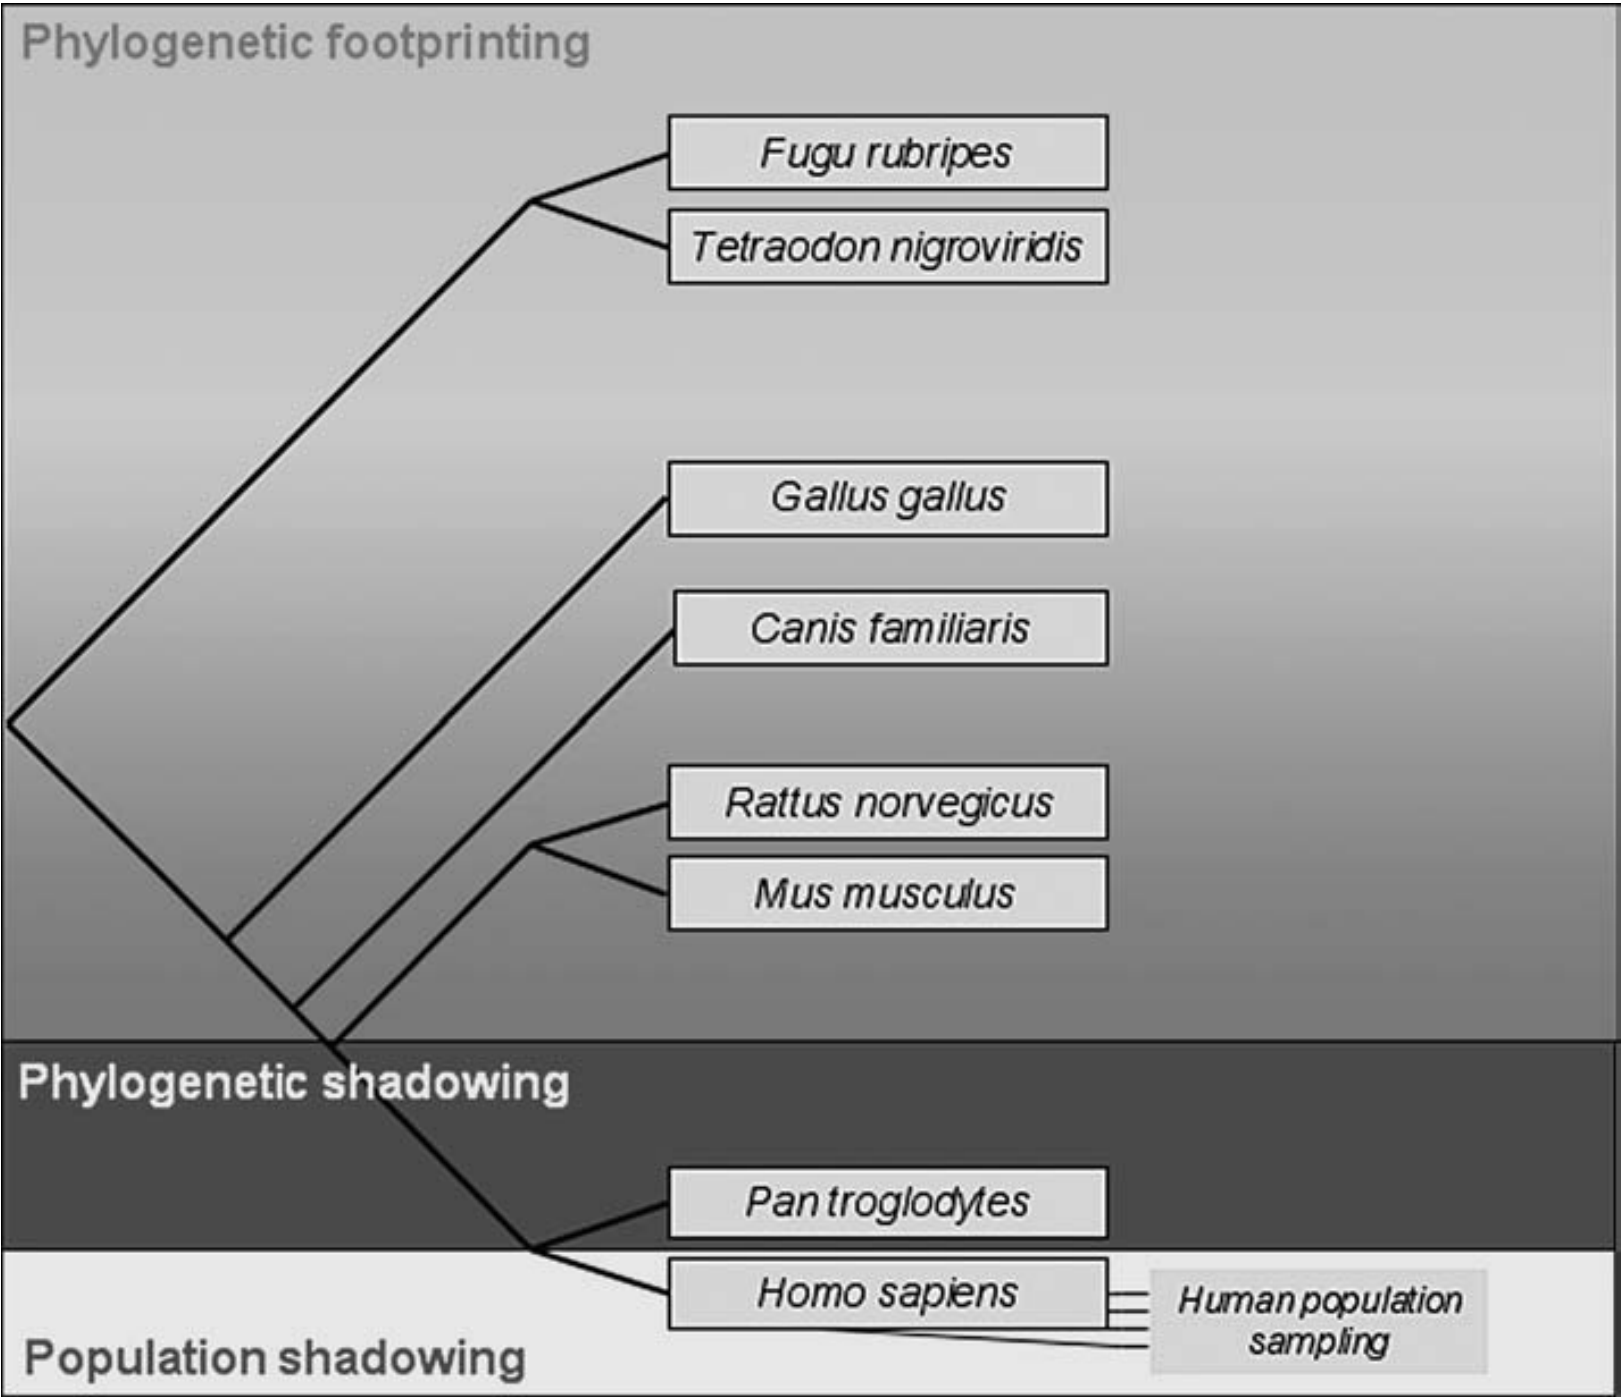
\includegraphics[scale=0.1]{images/phylo-shadowing}
      \end{figure}
	  \begin{itemize}
      %\item Phylogenetic Footprinting v/s Shadowing
      \item Selective pressure causes slower evolution of regulatory elements
      \item Phylogenetic footprinting -- Identifying highly consered sequences in evolutionary diverse species
      \item Need to explicitly model phylogenetic relationship over simple conservation based approaches
      \end{itemize}
\end{frame}
}


\begin{frame}[fragile]{Substitution Models}
\begin{itemize}
\item Evolution can be modeled as a continuous time markov chain. Transition Matrix $P(t) = \{P_{\alpha\beta}\}$
%\item $P'(t) = QP(t)$, where $Q$ is the mutation rate matrix 
\item Rate matrix $Q = \begin{pmatrix} * & \mu_{AC} & \mu_{AG} & \mu_{AT}\\
& & \cdots \end{pmatrix}$
\item $p_\alpha(t+\delta t) = p_\alpha(t) + \sum_{\beta \neq \alpha }\mu_{\beta \alpha}p_\beta(t) - \sum_{\beta  \neq \alpha}\mu_{\alpha \beta} p_\alpha(t)$
\item $P(t) = \exp(Qt)$
\item Simple models 
\begin{itemize}
\item Jukes Cantor (JC69): Equal base frequencies and equal mutation rates
\item Kimura (K80): Distinguishes between transition and transversion ratios
\item Felenstein (F81): Allows different base frequencies
\item HKY: Kimura+Felenstein
%\item Hasegawa Kishino  Yano (HKY85): Kimura  
\end{itemize}
\end{itemize}

\end{frame}

\begin{comment}
\begin{frame}[fragile]{Model Assumptions}
\begin{itemize}
\item Probability of fixation of a mutation $\alpha \rightarrow \beta$ is proportional to corresponding PWM entry. ($P(A_i=\alpha) = \theta_{i\alpha}$)
\item $P(s_i|A_i)$ is determined by using different substitution models which is our focus here
\end{itemize}
\end{frame}
\end{comment}


\begin{frame}[fragile]{Halpern Bruno Model : Accounting for position specific selection }
\begin{itemize}
\item Substitution v/s Mutation : Different things
\item JC/K80/F81: Do not explicitly differentiate mutation from selection
\item HB Model:
$$
\underbrace{r_{\alpha\beta}^{i}}_{\text{Substitution rate}}   =   \underbrace{\mu_{\alpha\beta}}_{\text{Probability of mutation(inst.)}} \times  \overbrace{f_{\alpha\beta}^i }^\text{Probability of fixation}
$$
\begin{itemize}
\item `Position-specific selection aware' substitution model, originally formulated for amino acids
\item All positions in the binding site evolve independently at equal rates
\item Covariation structure between different species are ignored
 
\end{itemize}
%\item Besides accounting for difference in equilbrium frequencies, it is also important to account for selection
%\item Effect of selection applies on probabilities of fixation once a mutation has occurred
%\item Fixation is rapid, allowing no time for polymorphism to exist
%\item Each base position evolves independently
%\item Only negative selection acts
%\item F81 considers evolutionary distance ignoring selection pressure
\end{itemize}

\end{frame}


\begin{frame}[fragile]{Halpern Bruno Model : Estimating fixation probability}
$$
{r_{\alpha\beta}^{i}}  =   {\mu_{\alpha\beta}} \times  {f_{\alpha\beta}^i }
$$
\begin{itemize}[<+- | alert@+>]
\item Selection coefficient($s$) -- Relative reduction in contribution of $\beta$ over $\alpha$ to fitness
$$F(\alpha)=1; F(\beta) = 1+s$$
\item Kimura's fixation probability: $f_{\alpha\beta} = \frac{1-e^{-2(F(\beta) - F(\alpha))}}{1-e^{-2N(F(\beta) - F(\alpha))}} = \frac{1-e^{-2s}}{1-e^{-2Ns}}$
\item Weak-mutation approximation($s<<1$): $f_{\alpha\beta} \approx \frac{2s}{1-e^{-2Ns}}$, $f_{\beta\alpha} \approx \frac{-2s}{1-e^{2Ns}}$
\item Reversibility condition: $\pi_\alpha \mu_{\alpha\beta}f_{\alpha\beta} = \pi_\beta \mu_{\beta\alpha} f_{\beta\alpha} \implies \frac{\pi_\beta \mu_{\beta\alpha}}{\pi_\alpha \mu_{\alpha\beta}} = \frac{f_{\alpha\beta}}{f_{\beta\alpha}} = e^{2Ns} $\\
\item $f_{\alpha\beta} \propto \frac{\ ln{\frac{\pi_\beta \mu_{\beta\alpha}  }{ \pi_\alpha \mu_{\alpha_\beta} } }} 
{1- \frac{ \pi_\alpha \mu_{\alpha_\beta} } {\pi_\beta \mu_{\beta\alpha} } } $  $\implies r_{\alpha\beta} = \mu_{\alpha\beta} \frac{\ln{\frac{\pi_\beta \mu_{\beta\alpha}}{\pi_\alpha \mu_{\alpha\beta}}}}{1-\frac{\pi_\alpha \mu_{\alpha\beta}  }{\pi_\alpha \mu_{\beta\alpha}  } } $
%\item \textbf{Key Insight} Greater difference in fitness $\implies$  less overall substitution
\end{itemize}
\end{frame}


\begin{frame}[fragile]{TFBS Prediction: Using HB Model over background}
	\begin{figure}
		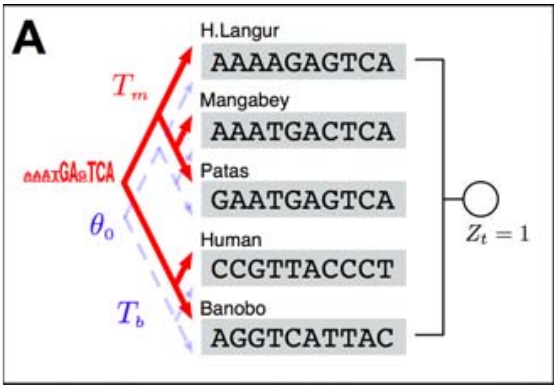
\includegraphics[width=0.77\textwidth]{images/monkey-model.png}
        \caption{Modeling full phylogeny as one component: \red{\textbf{{HB}}} or \blue{\textbf{JC/F81/HKY}}. $F(x| \theta) = \frac{\log P(S| \red{\textbf{{HB}}} ) }{ \log P(S|\blue{\textbf{JC}}) }$ }
	\end{figure}
\end{frame}

\begin{frame}[fragile]{HB model: Example with aligned sequences}
\footnotesize
\begin{figure}
    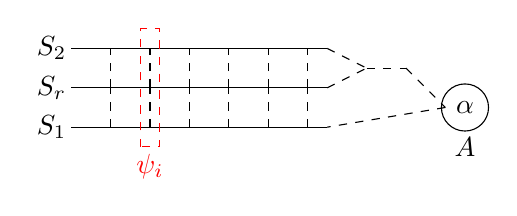
\begin{tikzpicture}[scale=0.5]
    \node at (0,0) (q1) {$S_1$};
    \node at (0,1) (q2) {$S_r$};    
    \node at (0,2) (q3) {$S_2$};    
        
    \draw (0.5,0) -- (7,0);
    \draw (0.5,1) -- (7,1);
    \draw (0.5,2) -- (7,2);
    \draw[dashed] (1.5,0) -- (1.5,1);
    \draw[dashed] (2.5,0) -- (2.5,1);
    \draw[dashed] (3.5,0) -- (3.5,1);
    \draw[dashed] (4.5,0) -- (4.5,1);
    \draw[dashed] (5.5,0) -- (5.5,1);
    \draw[dashed] (6.5,0) -- (6.5,1);
    
    \draw[dashed] (1.5,1) -- (1.5,2);
    \draw[dashed] (2.5,1) -- (2.5,2);
    \draw[dashed] (3.5,1) -- (3.5,2);
    \draw[dashed] (4.5,1) -- (4.5,2);
    \draw[dashed] (5.5,1) -- (5.5,2);
    \draw[dashed] (6.5,1) -- (6.5,2);
    
	\draw[dashed, red] (2.25,-0.5) rectangle (2.75,2.5);
    \node[red] at (2.5, -1) (q4) {$\psi_i$};
    
    \draw[dashed](7,2) -- (8,1.5);
    \draw[dashed](7,1) -- (8,1.5);
    \draw[dashed](8,1.5) -- (9,1.5);
    \draw[dashed](9,1.5) -- (10,0.5);
    \draw[dashed](10,0.5) -- (7,0);
    
    \node[circle, draw] at (10.5,0.5) {$\alpha$};
    \node at (10.5, -0.5) {$A$};
\end{tikzpicture}
\caption{\footnotesize MSA of Orthologous Sequences}
\end{figure}
   \begin{columns}[T,onlytextwidth]
    \column{0.5\textwidth}
      \begin{align*}       
        P(\psi_i) &= \sum_{\alpha }P(\psi_i, A_i=\alpha | \theta)\\  
        &= \sum_\alpha P(A_i=\alpha)P(\psi_i| A_i=\alpha,\theta) \\ 
        &= \sum_\alpha P(A_i=\alpha)\prod_{s_i}\highlight{P(s_i| A_i=\alpha,\theta) }\\ 
        %&= \sum_{\alpha} \theta_{i\alpha}\prod_{k=1}^K P_{\alpha s_{i}^k}\\
      \end{align*}
      \column{0.5\textwidth}
      \begin{align*}
    	S &= \{\psi_1, \psi_2, \dots, \psi_L\};\\
        \psi_i &= \{s_1^i, s_2^i, \dots, s_N^i\}\\
        A &= \text{Unobserved ancestral sequence}\\
		%a\theta_{i\alpha} &= \text{$i^{th}$ PWM entry for base $\alpha$}\\
        %P_{\alpha S_i^k} &= \text{$k^{th}$ base of $i^{th}$ sequence}
		\end{align*}
 	 \end{columns}
     
\end{frame}



\section{Site Level Selection}



\begin{frame}[fragile]{Selection acting on whole TFBS as a unit}
\begin{itemize}[<+- | alert@+>]
\item Substitution rates are position specific in TFBS but independence assumption does not necessarily hold
%\item Core regions of TF should be under stronger selection constraints 
\item Intuition: A TFBS will retain functionality if it is close enough to optimality even if a crucial nucleotide undergoes substitution (and eventually getting fixed)
\item The same substitution in a far less optimal site might lead to a functional loss
\item A better model would be to account for substitution of entire site i.e. site-level selection treating binding sites as evolutionary units
%\item The site is functional if it is below a certain energy threshold (bindin
\item How: Reformulate the previous problem for two sites $a,b$ instead of bases
\end{itemize}
\end{frame}


\section{Functional Turnover}

\begin{frame}[fragile]{TFBS Turnover}
\begin{figure}
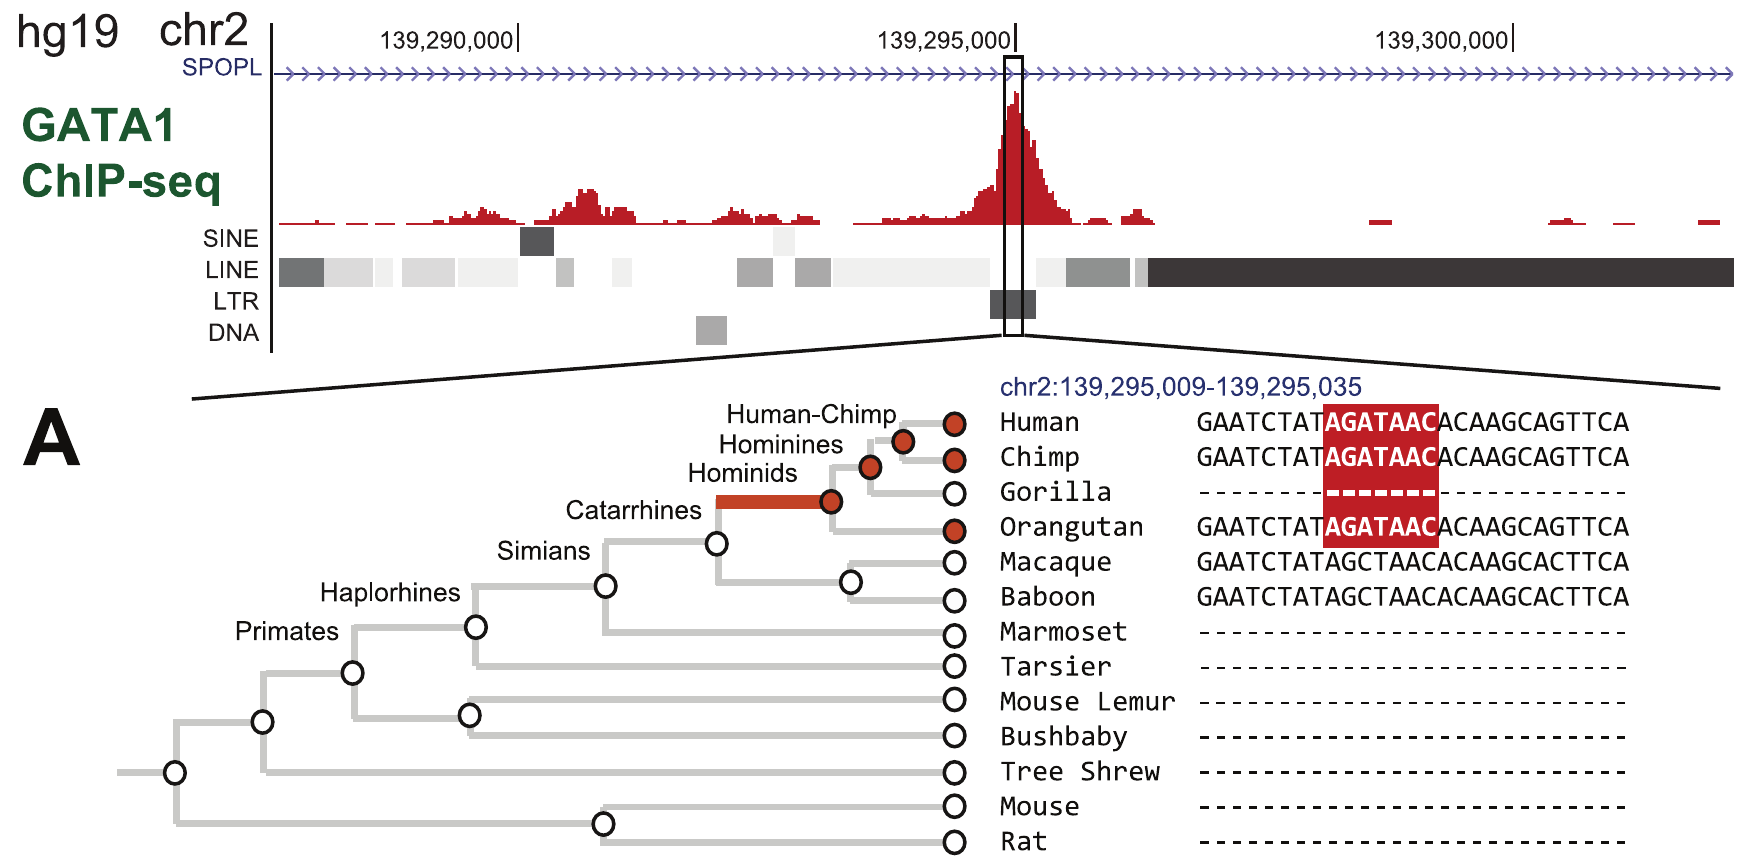
\includegraphics[width=\textwidth]{images/branchorigin}
\caption{Functional turnover: TFBS can be gained or lost during evolution}
\end{figure}
\end{frame}

\begin{frame}[fragile]{Functional turnover: Birth \& Death Process}
Aim: Detect lineage-specific rates of TFBS evolution and the branch of origin of individual TFBS
\begin{itemize}
\item Binding sites are known to show turnover: TFBS can be gained/lost during speciation events 
\item Estimate rate of birth $\alpha$ and death $\beta$ from orthologous sequences
\item Infer ancestral states; branch of origin %n contrast to conservation based approaches, use birth-death model to i
\end{itemize}
\end{frame} 

\begin{frame}[fragile]{Functional turnover: Birth \& Death Process}
\begin{align*}
w(t) &= \text{Probability that TFBS exists at time $t$}\\
\alpha,\beta &= \text{Birth, death rate respectively}\\
w(t+1) &= \alpha(1-w(t)) + (1-\beta) w(t)\\
w'(t) &= \alpha - (\alpha+\beta) w(t)
\end{align*}

We formulate two type of solutions, $u(t), v(t)$ such that: $u(t)$ represents those class of motifs present at $t=0$
and $v(t)$ represents class of motifs that did not exist at $t=0$.
\end{frame} 

\begin{frame}[fragile]{Functional turnover: Birth \& Death Process}
Let $p_{ij}(t)$ represent the probability of observing $j$ motif occurrences after $t$ , initial $i$
\begin{align*}
u(t) &= \frac{1}{\alpha+\beta} (\alpha + \beta e^{-(\alpha+\beta)t})\\
v(t) &= \frac{\alpha}{\alpha+\beta} (1-e^{-(\alpha+\beta)t})\\
%U_{i,k}(t) &= \frac{i!}{(i-k)!k!}{u(t)}^k(1-u(t))^{i-k}\\
%V_{N-i,b}(t) &= \frac{(N-i)!}{(N-i-b)!b!} {v(t)}^b (1-v(t))^{N-i-b}\\
%p_{i,j}(t) &= \sum_{k=0}^{\min{i,j}} U_{i,k}(t) V_{N-i,j-k}(t)
\end{align*}
\begin{itemize}
\item At each node calculate the likelihood of observing daughter nodes given $\alpha, \beta$
\item Determine most likely ancestral state using MLE
\item Infer branch of origin
\end{itemize}
\end{frame} 






\begin{comment}


\begin{frame}[fragile]{Problem with Phylogenetic Shadowing based approaches}
\begin{itemize}
\item Two main assumptions on approaches so far:
\begin{itemize}
\item Independence: Sites evolve independently
\item Completeness: Orthology as captured by MSA complete
\end{itemize}
\item Unlike genes, TFBS exhibit frequent turnover 
\end{itemize}
Assumptions make modeling easier, works well for gene coding regions in closesly related taxa since in genes turnover 
PhyME, MONKEY do not offer any insight into evolutionars dyanmics of motif turnover.
\end{frame}
\end{comment}




\begin{comment}
\begin{frame}[fragile]{Birth-Death model: Where's the branch}
\begin{figure}
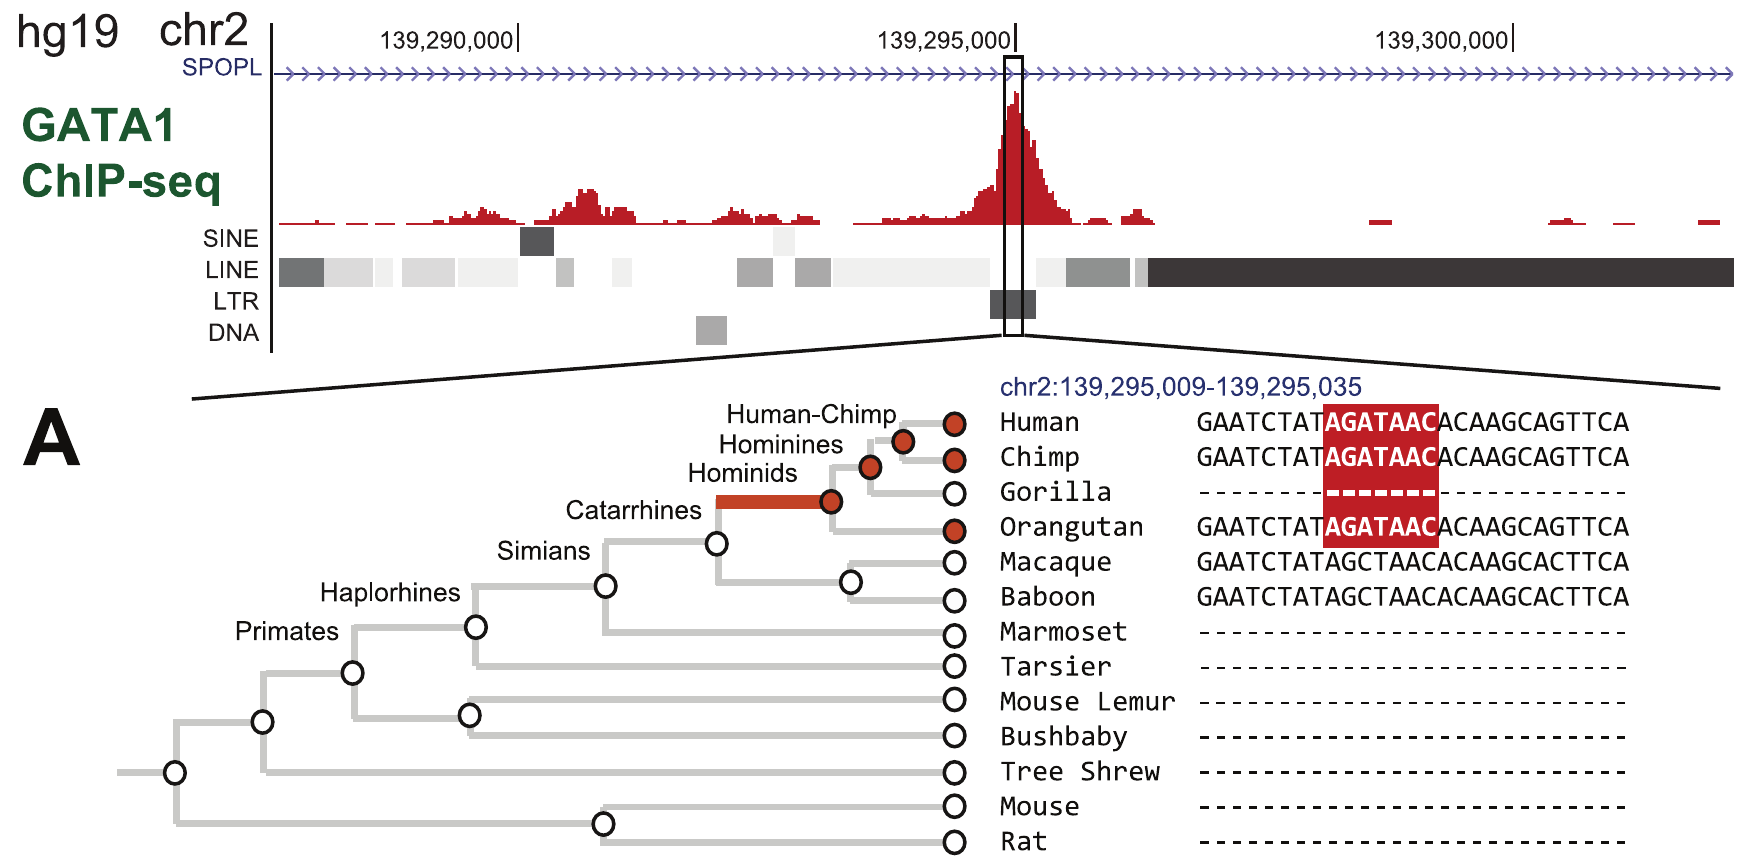
\includegraphics[width=\linewidth]{images/branchorigin.png}
\caption{Phylogenies in the birth-death model framewrok}
\end{figure}

\end{frame}
\end{comment}


 \section{ (Lineage/Specie) specific models}




\begin{comment}

\end{}
\begin{frame}[fragile]{Lineage Specific Evolution}
\begin{figure}
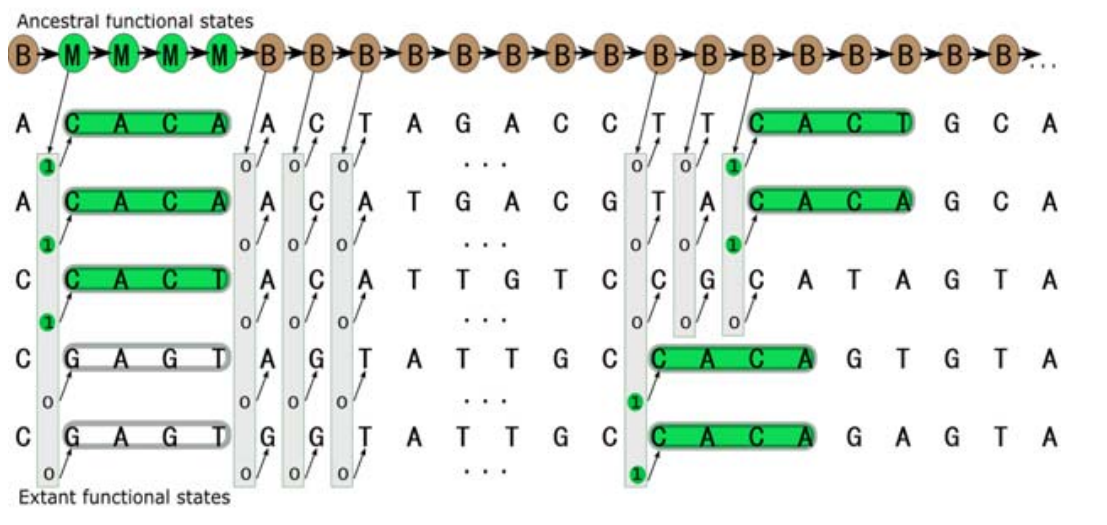
\includegraphics[width=\linewidth]{images/csmet2.png}
\end{figure}
Ancestor = background $\implies$ evolution independent\\ 
Ancestor =  motif $\implies$ TFBS evolves as unit
\end{frame}

\end{comment}


\begin{frame}[fragile]{Full phylogeny evolving following motif model}
    \begin{figure}
%    \begin{tikzpicture}[scale=0.5]
\begin{forest}
%    red subtree/.style={for tree={text=red},for descendants={edge=red}}}
label/.style={text=black},
sn edges/.style={for tree={
parent anchor=south, child anchor=north}, text=black},
sn edges
[$\alpha_0$ ,s sep=15mm, for tree=draw
    [$\alpha_1$ , l*=2,  edge label={node[midway,left,font=\scriptsize] {$P_{\alpha_0 \alpha_1}$}} , edge={dashed, red}
      [$s_1$, edge label={node[midway,left,font=\scriptsize] {$P_{\alpha_1 s_1}$}} , edge={dashed, red}] 
      [$s_2$, edge label={node[midway,right,font=\scriptsize] {$P_{\alpha_1 s_2}$}}, edge={dashed, red} ]
    ]
    [$\alpha_2$, edge label={node[midway,right,font=\scriptsize] {$P_{\alpha_0 \alpha_2}$}}, s sep= 12mm, edge={dashed, red}
      [$\alpha_3$, edge label={node[midway,left,font=\scriptsize] {$P_{\alpha_2\alpha_3}$}}, edge={dashed, red}
      	[$s_3$, edge label={node[midway,left,font=\scriptsize] {$P_{\alpha_2\alpha_3}$}}, edge={dashed, red}]
      	[$s_4$, edge label={node[midway,right,font=\scriptsize] {$P_{\alpha_2\alpha_3}$}}, edge={dashed, red}]      
      ] 
      [$\alpha_4$, edge label={node[midway,right,font=\scriptsize] {$P_{\alpha_2\alpha_4}$}}, edge={dashed, red}
      	[$s_5$, edge label={node[midway,left,font=\scriptsize] {$P_{\alpha_4s_5}$}}, edge={dashed, red}]
      	[$s_6$, edge label={node[midway,right,font=\scriptsize] {$P_{\alpha_5s_6}$}}, edge={dashed, red}]
      ]
  ] 
]
\end{forest}
%\end{tikzpicture}
\end{figure}


\end{frame}

\begin{frame}[fragile]{Full phylogeny evolving following background model}
\begin{figure}

\begin{forest}
%    red subtree/.style={for tree={text=red},for descendants={edge=red}}}
label/.style={text=black},
sn edges/.style={for tree={
parent anchor=south, child anchor=north}, text=black},
sn edges
[$\alpha_0$ ,s sep=15mm, for tree=draw
    [$\alpha_1$ , l*=2,  edge label={node[midway,left,font=\scriptsize] {$P_{\alpha_0 \alpha_1}$}} 
      [$s_1$, edge label={node[midway,left,font=\scriptsize] {$P_{\alpha_1 s_1}$}} ] 
      [$s_2$, edge label={node[midway,right,font=\scriptsize] {$P_{\alpha_1 s_2}$}} ]
    ]
    [$\alpha_2$, edge label={node[midway,right,font=\scriptsize] {$P_{\alpha_0 \alpha_2}$}}, s sep= 12mm
      [$\alpha_3$, edge label={node[midway,left,font=\scriptsize] {$P_{\alpha_2\alpha_3}$}}
      	[$s_3$, edge label={node[midway,left,font=\scriptsize] {$P_{\alpha_2\alpha_3}$}}]
      	[$s_4$, edge label={node[midway,right,font=\scriptsize] {$P_{\alpha_2\alpha_3}$}}]      
      ] 
      [$\alpha_4$, edge label={node[midway,right,font=\scriptsize] {$P_{\alpha_2\alpha_4}$}}
      	[$s_5$, edge label={node[midway,left,font=\scriptsize] {$P_{\alpha_4s_5}$}}]
      	[$s_6$, edge label={node[midway,right,font=\scriptsize] {$P_{\alpha_5s_6}$}}]
      ]
  ] 
]
\end{forest}
\end{figure}

\end{frame}



\begin{frame}[fragile]{Lineage Specific Evolution}
\begin{figure}
\centering
\begin{forest}
%    red subtree/.style={for tree={text=red},for descendants={edge=red}}}
label/.style={text=black},
sn edges/.style={for tree={
parent anchor=south, child anchor=north}, text=black},
sn edges
[$\alpha_0$ ,s sep=15mm, for tree=draw
    [$\alpha_1$ , l*=2,  edge label={node[midway,left,font=\scriptsize] {$P_{\alpha_0 \alpha_1}$}} 
      [$s_1$, edge label={node[midway,left,font=\scriptsize] {$P_{\alpha_1 s_1}$}} ] 
      [$s_2$, edge label={node[midway,right,font=\scriptsize] {$P_{\alpha_1 s_2}$}} ]
    ]
    [$\alpha_2$, edge label={node[midway,right,font=\scriptsize] {$P_{\alpha_0 \alpha_2}$}}, s sep= 12mm, edge={dashed, red}
      [$\alpha_3$, edge label={node[midway,left,font=\scriptsize] {$P_{\alpha_2\alpha_3}$}}, edge={dashed, red}
      	[$s_3$, edge label={node[midway,left,font=\scriptsize] {$P_{\alpha_2\alpha_3}$}}, edge={dashed, red}]
      	[$s_4$, edge label={node[midway,right,font=\scriptsize] {$P_{\alpha_2\alpha_3}$}}, edge={dashed, red}]      
      ] 
      [$\alpha_4$, edge label={node[midway,right,font=\scriptsize] {$P_{\alpha_2\alpha_4}$}}, edge={dashed, red}
      	[$s_5$, edge label={node[midway,left,font=\scriptsize] {$P_{\alpha_4s_5}$}}, edge={dashed, red}]
      	[$s_6$, edge label={node[midway,right,font=\scriptsize] {$P_{\alpha_5s_6}$}}, edge={dashed, red}]
      ]
  ] 
]
\end{forest}
\end{figure}

\end{frame}


\begin{frame}[fragile]{Specie Specific Evolution}
\begin{figure}
\centering
\begin{forest}
%    red subtree/.style={for tree={text=red},for descendants={edge=red}}}
label/.style={text=black},
sn edges/.style={for tree={
parent anchor=south, child anchor=north}, text=black},
sn edges
[$\alpha_0$ ,s sep=15mm, for tree=draw
    [$\alpha_1$ , l*=2,  edge label={node[midway,left,font=\scriptsize] {$P_{\alpha_0 \alpha_1}$}} 
      [$s_1$, edge label={node[midway,left,font=\scriptsize] {$P_{\alpha_1 s_1}$}} ] 
      [$s_2$, edge label={node[midway,right,font=\scriptsize] {$P_{\alpha_1 s_2}$}} ]
    ]
    [$\alpha_2$, edge label={node[midway,right,font=\scriptsize] {$P_{\alpha_0 \alpha_2}$}}, s sep= 12mm, edge={dashed, red}
      [$\alpha_3$, edge label={node[midway,left,font=\scriptsize] {$P_{\alpha_2\alpha_3}$}}, edge={dashed, red}
      	[$s_3$, edge label={node[midway,left,font=\scriptsize] {$P_{\alpha_2\alpha_3}$}}, edge={dashed, red}]
      	[$s_4$, edge label={node[midway,right,font=\scriptsize] {$P_{\alpha_2\alpha_3}$}}]      
      ] 
      [$\alpha_4$, edge label={node[midway,right,font=\scriptsize] {$P_{\alpha_2\alpha_4}$}}
      	[$s_5$, edge label={node[midway,left,font=\scriptsize] {$P_{\alpha_4s_5}$}}]
      	[$s_6$, edge label={node[midway,right,font=\scriptsize] {$P_{\alpha_5s_6}$}}]
      ]
  ] 
]
\end{forest}
\end{figure}

\end{frame}

\begin{frame}[fragile]{Lineage Specific Evolution}
\begin{figure}
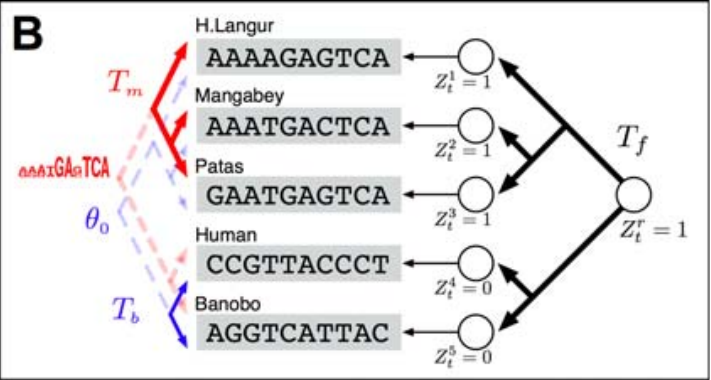
\includegraphics[width=\linewidth]{images/csmet-model.png}
\caption{Lineage specific model}
\end{figure}
\end{frame}

\begin{frame}[fragile]{Lineage Specific Evolution: Model}
\begin{itemize}
\item Explicitly model functional turnover long $T_f$ as a JC substitution process 
%$$\beta = \mu \times T$$
$$ P_f = \begin{pmatrix}
\frac{1}{2} + \frac{1}{2} e^{-2\beta} & \frac{1}{2} - \frac{1}{2} e^{-2\beta}\\
\frac{1}{2} - \frac{1}{2} e^{-2\beta} & \frac{1}{2} + \frac{1}{2} e^{-2\beta}
\end{pmatrix}$$ 
$ \beta = $ branch length
\item Conditioning on TFBS functionality to model nucleotide substitution
\item Capture function-specific evolution in every lineage
\end{itemize}
\end{frame}


\begin{frame}{Summary}
\begin{itemize}
\item HB model accounts for selection in TFBS evolution 
\item HB model can be extended to allow TFBS as a unit of evolution
\item Turnovers can be treated in birth-death framework
\item More general models can account for turnover and functional dependency across lineages
\end{itemize}
\end{frame}

\begin{frame}[standout]
  Questions?
\end{frame}

\appendix

\begin{frame}[allowframebreaks]{Ornstein-Uhlenbeck Model}
\begin{itemize}
\item HB models neglects lineage or specie specific selection
\item OU models this gap by accounting for lineage/specie specific selection by requiring regime specific optima to be obtained
%\item OU models can account for whole element substitution by defining a quantitative trait as a score attached to the TFBS: $X(t)$
\item OU models can model evolution by defining a quantitative trait as a score attached to the TFBS: $X(t)$
\item Motivation: Account for the optima in the phylogeny regime assuming the change in optima coincide with phylogenetic branch points
\item $X(t)$ evolves by two components one deterministic(selection), other stochastic (mutation)
\end{itemize}
\begin{align*}
dX(t) &= \alpha(\theta-X(t)) + \sigma dB(t)\\
\alpha & = \text{Strength of selection}\\
\theta - X(t) & = \text{Distance from optimum value}\\
\sigma &= \text{strength of random drift}\\
dB(t) &= \text{random white noise}
\end{align*}
Farther the TFBS from `optimum' $\implies$ higher the selection force\\
%OU mjodels are the only non-trivial Gauss-Markov process
\end{frame}

\begin{frame}[fragile]{Ornstein-Uhlenbeck Model: Multivariate normal}
   \begin{columns}[T,onlytextwidth]
    \column{0.3\textwidth}
	\begin{figure}
    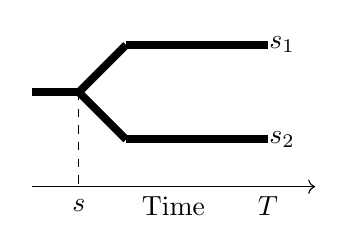
\begin{tikzpicture}[scale=0.6]
    \tikzstyle{operator} = [draw,fill=white,minimum size=1em] 
        \draw[->] (0,-2) -- (6,-2);
        \draw[line width=1mm] (0,0) -- (1,0);   
        \draw[line width=1mm] (1,0) -- (2,1);
        \draw[line width=1mm] (2,1) -- (5,1);
        \draw[line width=1mm] (1,0) -- (2,-1);
        \draw[line width=1mm] (2,-1) -- (5,-1);   
        \draw[dashed] (1,0) -- (1,-2);
        \node at (1,-2.4) {$s$};
        \node at (3,-2.4) {Time};
        \node at (5,-2.4) {$T$};
        \node at (5.3,1) {$s_1$};
        \node at (5.3,-1) {$s_2$};
    \end{tikzpicture}
\caption{$s_1$, $s_2$ -- BM}    
\end{figure}

	\column{0.7\textwidth}    
    \begin{align*}
E[\mathbf{X}(t)] &= \begin{pmatrix}
\theta_0\\
\theta_1
\end{pmatrix}\\
 \texorpdfstring{{\Sigma}} &= \sigma^2\begin{pmatrix}
T & s\\
s & T
\end{pmatrix}\\
\end{align*}    
  \end{columns}
  \begin{columns}[T,onlytextwidth]
    \column{0.3\textwidth}     
    \begin{figure}
    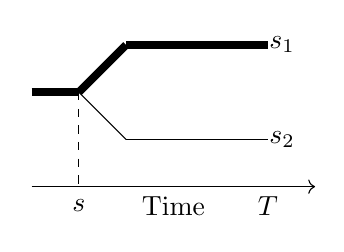
\begin{tikzpicture}[scale=0.6]
    \tikzstyle{operator} = [draw,fill=white,minimum size=1em] 
        \draw[->] (0,-2) -- (6,-2);
        \draw[line width=1mm] (0,0) -- (1,0);   
        \draw[line width=1mm] (1,0) -- (2,1);
        \draw[line width=1mm] (2,1) -- (5,1);
        \draw (1,0) -- (2,-1);
        \draw (2,-1) -- (5,-1);   
        \draw[dashed] (1,0) -- (1,-2);
        \node at (1,-2.4) {$s$};
        \node at (3,-2.4) {Time};
        \node at (5,-2.4) {$T$};
        \node at (5.3,1) {$s_1$};
        \node at (5.3,-1) {$s_2$};
    \end{tikzpicture}
    \caption{$s_2$ -- new optimum regime, $s_1$ -- ancestral}    
\end{figure}
    \column{0.7\textwidth}
    \begin{align*}
      E[X_1(T)] &= \theta_0e^{-\alpha T}+ \theta_1(1-e^{-\alpha T})\\
      E[X_2(T)] &= \theta_0e^{-\alpha T} + \theta_1e^{-\alpha(T-s)}(1-e^{-\alpha s})\\ 
      &+ \theta_2(1-e^{-\alpha(T-s)})\
	\end{align*}
  \end{columns}
\end{frame}


\begin{frame}[allowframebreaks]{Jukes Cantor / HKY / F81}
Jukes Cantor
\begin{align*}
Q &= \begin{pmatrix}
-\frac{3\mu}{4} & \frac{\mu}{4} & \frac{\mu}{4} & \frac{\mu}{4}\\
\frac{\mu}{4} & -\frac{3\mu}{4} &  \frac{\mu}{4} & \frac{\mu}{4}\\
\frac{\mu}{4} & \frac{\mu}{4} &  -\frac{3\mu}{4} & \frac{\mu}{4}\\
\frac{\mu}{4} & \frac{\mu}{4} & \frac{\mu}{4} & -\frac{3\mu}{4}\\
\end{pmatrix}\\
P &= \begin{pmatrix}
\frac{1}{4}+\frac{3}{4}e^{-t\mu} & \frac{1}{4}-\frac{3}{4}e^{-t\mu} & \frac{1}{4}-\frac{3}{4}e^{-t\mu} & \frac{1}{4}-\frac{3}{4}e^{-t\mu}\\
\frac{1}{4}-\frac{1}{4}e^{-t\mu} & \frac{1}{4}+\frac{3}{4}e^{-t\mu} & \frac{1}{4}-\frac{1}{4}e^{-t\mu} & \frac{1}{4}-\frac{1}{4}e^{-t\mu}\\
\frac{1}{4}-\frac{1}{4}e^{-t\mu} & \frac{1}{4}-\frac{1}{4}e^{-t\mu} & \frac{1}{4}+\frac{3}{4}e^{-t\mu} & \frac{1}{4}-\frac{1}{4}e^{-t\mu}\\
\frac{1}{4}-\frac{1}{4}e^{-t\mu} & \frac{1}{4}-\frac{1}{4}e^{-t\mu} & \frac{1}{4}-\frac{1}{4}e^{-t\mu} & \frac{1}{4}+\frac{3}{4}e^{-t\mu}\\
\end{pmatrix}
\end{align*}
\end{frame}


\begin{frame}[fragile]{Lineage Specific Evolution}
\begin{figure}
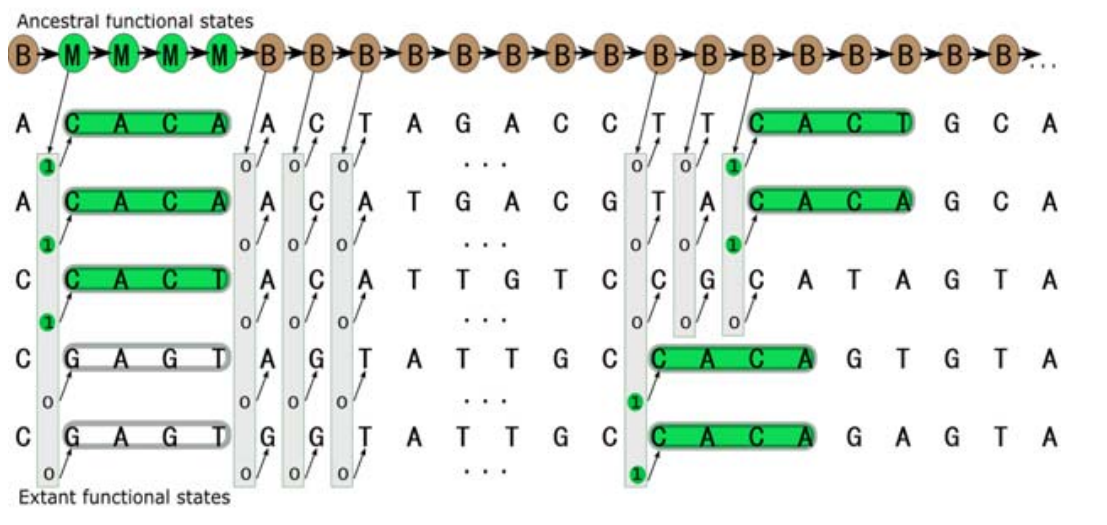
\includegraphics[width=\linewidth]{images/csmet2.png}
\end{figure}
Ancestor = background $\implies$ evolution independent\\ 
Ancestor =  motif $\implies$ TFBS evolves as unit
\end{frame}




\end{document}
